\documentclass[journal]{IEEEtran}
\def\BibTeX{{\rm B\kern-.05em{\sc i\kern-.025em b}\kern-.08em
    T\kern-.1667em\lower.7ex\hbox{E}\kern-.125emX}}

\usepackage{amsmath}
\usepackage{bm}
\usepackage{nicefrac}
\usepackage{booktabs}
\usepackage{array}
\usepackage{multirow}
\usepackage{threeparttable}
\usepackage{makecell}
\usepackage[procnumbered,ruled,vlined,linesnumbered]{algorithm2e}
\usepackage{siunitx}
\usepackage{stfloats}
\usepackage{graphicx}
\usepackage{subfigure}
\usepackage{hyperref}
\usepackage{array}
\usepackage{epstopdf}
\usepackage{balance}
\usepackage{tabularx}
\usepackage{stfloats}
\usepackage{lipsum}

\newtheorem{problem}{Problem}
\newtheorem{theorem}{Theorem}[section]
\newtheorem{corollary}[theorem]{Corollary}
\newtheorem{lemma}[theorem]{Lemma}
\newtheorem{definition}[theorem]{Definition}
\newtheorem{fact}[theorem]{Fact}

% \newcommand{\proof}{{\bf Proof.}\hskip 0.3truecm}
% \newcommand{\endproof}{\quad \(\Box\)}

\newcommand{\defeq}{\stackrel{\mathrm{def}}{=}}
\newcommand{\setof}[1]{\left\{#1 \right\}}
% \newcommand{\sizeof}[1]{\left|#1 \right|}
\newcommand{\abs}[1]{\left|#1 \right|}
\newcommand{\mean}[1]{\mathbb{E}[#1]}
\newcommand{\ceil}[1]{\left\lceil#1\right\rceil}
\newcommand{\Abs}[1]{\left\Vert#1\right\Vert}
\newcommand{\trace}[1]{\mathrm{Tr}\left(#1\right)}

\newcommand{\bsym}[1]{\boldsymbol{#1}}
\newcommand{\myord}[1]{{#1}^{\rm{th}}}
\newcommand{\rea}{\mathbb{R}}
\newcommand{\gr}{\mathcal{G}}
\newcommand{\vecd}{\bsym{d}}
\newcommand{\veca}{\bsym{a}}
\newcommand{\vecb}{\bsym{b}}
\newcommand{\vece}{\bsym{e}}
\newcommand{\allone}{\bsym{1}}
\newcommand{\vecl}{\bsym{l}}
\newcommand{\vecv}{\bsym{v}}
\newcommand{\vecpi}{\bsym{\pi}}
\newcommand{\vecx}{\bsym{x}}

\newcommand{\pscr}{\mathscr{P}}

\newcommand{\lap}{\bsym{L}}
\newcommand{\matd}{\bsym{D}}
\newcommand{\mata}{\bsym{A}}
\newcommand{\matb}{\bsym{B}}
\newcommand{\matw}{\bsym{W}}
\newcommand{\matp}{\bsym{P}}
\newcommand{\matpcal}{\bsym{\mathcal{P}}}
\newcommand{\matf}{\bsym{F}}
\newcommand{\matfstar}{\bsym{F}^*}
\newcommand{\mati}{\bsym{I}}
\newcommand{\matq}{\bsym{Q}}
\newcommand{\matr}{\bsym{R}}
\newcommand{\mats}{\bsym{S}}
\newcommand{\matx}{\bsym{X}}
\newcommand{\maty}{\bsym{Y}}
\newcommand{\matz}{\bsym{Z}}
\newcommand{\matpi}{\bsym{\Pi}}

\newcommand{\lemref}[1]{Lemma~\ref{#1}}
\newcommand{\thmref}[1]{Theorem~\ref{#1}}
\newcommand{\probref}[1]{Problem~\ref{#1}}
\newcommand{\algoref}[1]{Algorithm~\ref{#1}}
\newcommand{\defref}[1]{Definition~\ref{#1}}
\newcommand{\secref}[1]{Section~\ref{#1}}
\newcommand{\tabref}[1]{Table~\ref{#1}}
\newcommand{\figref}[1]{Figure~\ref{#1}}

\newcommand{\edge}[2]{\langle #1, #2 \rangle}


\DeclareMathOperator*{\argmin}{arg\,min}
\DeclareMathOperator*{\argmax}{arg\,max}

\DontPrintSemicolon
\SetKw{KwAnd}{and}
\SetFuncSty{textsc}
\SetKwInOut{Input}{Input\ \ \ \ }

\SetKwInOut{Output}{Output}
\newcommand{\todo}[1]{{\bf \color{red} TODO: #1}}

\begin{document}

\title{Absorbing Time of Random Walks\\ as a Node Group Centrality}
\author{Haisong~Xia,
    Zuobai~Zhang,
    Xiaotian~Zhou,
    Zhuoqing~Song,
    Zhongzhi~Zhang~\IEEEmembership{Member,~IEEE}
    \thanks{Haisong Xia, Xiaotian Zhou and Zhongzhi Zhang are with the Shanghai Key Laboratory of Intelligent Information Processing, School of Computer Science, Fudan University, Shanghai 200433, China;Zhongzhi Zhang and Haibin Kan are also with the Shanghai Engineering Research Institute of Blockchain, Shanghai 200433, China.}
}

\maketitle

\begin{abstract}
    For random walks on a graph, the mean hitting time \(H_j\) from a vertex \(i\) chosen from the stationary distribution to the target vertex \(j\) can be used as a measure of importance for vertex \(j\), while the Kemeny constant \(K\) is the mean hitting time from a vertex \(i\) to a vertex \(j\) selected randomly according to the stationary distribution.
    Both quantities have found a large variety of applications in different areas.
    However, their high computational complexity limits their applications, especially for large networks with millions of vertices.
    In this paper, we first establish a connection between the two quantities, representing \(K\) in terms of \(H_j\) for all vertices.
    Subsequently, we extend the notion of mean hitting time to the case of multiple vertices, proposing a vertex group centrality and its minimization problem.
    We then express these quantities in terms of either the pseudoinverse for graph Laplacian or the inverse for a SDDM matrix, based on which we develop an efficient algorithm that provides an approximation of \(H_j\) for all vertices and \(K\) in nearly linear time with respect to the edge number, with high probability.
    Based on the aforementioned algorithm, we provide another nearly linear greedy algorithm to solve the minimization problem of our proposed vertex group centrality with a \(1-\frac{k}{k-1}\cdot\frac{1}{e}-\epsilon\) approximate factor for any \(\epsilon\in(0,1)\).
    Extensive experiment results on real-life and model networks validate both the efficiency and accuracy of our proposed algorithms.
\end{abstract}

\begin{IEEEkeywords}
    Random walk, hitting time, Kemeny constant, spectral algorithm, complex network, vertex centrality.
\end{IEEEkeywords}

\section{Introduction}\label{sec:intro}

\IEEEPARstart{A}{s} a powerful tool and method, random walks have found broad applications in various aspects.
Frequently cited examples include image segmentation~\cite{Le06}, random algorithm design~\cite{SaDi12}, collaborative recommendation~\cite{FoPiReSa07}, community detection~\cite{LaDeBa14}, among others.
A fundamental quantity related to random walks is hitting time~\cite{Lo93}, also called first-passage time~\cite{CoBeTeVoKl07}.
For a random walk on a graph, the hitting time \(H_{ij}\) from a vertex \(i\) to another vertex \(j\) is the expected time for the walker starting from \(i\) to visit \(j\) for the first time.
Hitting time is related to many problems and has been successfully applied to diverse areas, such as Hanoi problem with random move~\cite{WuZhCh11}, query suggestion~\cite{MeZhCh08}, and clustering algorithm~\cite{ChLiTa08}.

Except for the intrinsic interest of hitting time itself and its direct applications, many other relevant quantities related to random walks are encoded in or expressed in terms of this crucial quantity, for example, absorbing random-walk centrality~\cite{MaMagi15} (or Markov centrality~\cite{WhSm03}), Kemeny constant~\cite{Hu14} and random detour time~\cite{RaZh13}.
As the name implies, the absorbing random-walk centrality is a measure for the importance of vertices on a graph.
For a vertex \(j\), its absorbing random-walk centrality \(H_j\) is defined by \(H_j=\sum_{i} \rho(i) H_{ij}\), where \(\rho(\cdot)\) is the starting probability distribution over all vertices.
Different from the shortest-path based centrality measures, random-walk based centrality metrics include the contributions from essentially all paths~\cite{Ne05}, and thus have a better discriminating power.

For random walks on a graph with \(n\) vertices, the Kemeny constant \(K\) is defined as the expected time for the walker starting from one vertex to second vertex selected randomly from the graph according to the stationary distribution \(\vecpi=\left(\pi_1, \pi_2, \cdots, \pi_n\right)^{\top}\) of the random walk, that is, \(K=\sum_{j} \pi_j H_{ij}\).
The Kemeny constant has also found a wealth of applications in different fields~\cite{Hu14}.
It can be utilized to gauge the efficiency of user navigation through the World Wide Web (WWW)~\cite{LeLo02}.
Moreover, the Kemeny constant is related to the mixing rate of an irreducible Markov chain~\cite{LePeWi09}, by regarding it as the expected time to mixing of the Markov chain~\cite{Hu06}.
Recently, the Kemeny constant has been applied to measure the efficiency of robotic surveillance in network environments~\cite{PaAgBu15} and to characterize the noise robustness of a class of protocols for formation control~\cite{JaOl15}

Despite the wide range of applications of the absorbing random-walk centrality and the Kemeny constant, it is a computational challenge to obtain their exact values.
By definition, both the absorbing random-walk centrality and the Kemeny constant are a partial average of some hitting times.
However, the exact value of hitting time between any pair of vertices in a graph involves all eigenvalues and eigenvectors of (normalized) Laplacian matrix associated with the graph~\cite{Lo93,LiZh13PRE}, the computation complexity of which is the cube of the vertex number.
Thus, for large realistic networks with millions of vertices, we cannot obtain their absorbing random-walk centrality and the Kemeny constant by resorting this straightforward method for computing hitting time.
It is then of theoretical and practical interest to seek for alternative approximate approaches that scale to large networks.

While computing absorbing random-walk centrality for a single vertex can be difficult, it is even more complex to find a group of \(k\) important vertices, which arises in many studies.
For instance, in the field of wireless networks, sensor placement involves selecting an optimal subset of vertices to place sensors to sample physical signals~\cite{KrSiGu08,RaChVe13}, such as radiation or temperature.
Another example is point cloud sampling~\cite{DiChWaBa20,ChTiFeVeKo17}, which requires selecting a representative subset of points to preserve the geometric features of reconstruction.
Traditional methods of ranking individual vertices may not meet these requirements, making it necessary to propose a vertex group centrality.

We introduce a new vertex group centrality called Absorbing Group Centrality (AGC) by extending absorbing random-walk centrality to the case of multiple vertices.
For a connected undirected graph and a vertex group \(S\), AGC \(\manc{S}\) is the expected hitting time for a random walker starting from a vertex \(u\) to an arbitary vertex in \(S\). Here, vertex \(u\) is chosen based on the stationary distribution \(\vecpi\).
We also introduce the AGC minimization problem, which involves identifying the vertex group \(S^*\) with capacity \(k\) that minimizes AGC \(\manc{S^*}\).

In this paper, we present algorithms that can address the following tasks in large networks with nearly linear time complexity:
\begin{itemize}
    \item Computing absorbing random-walk centrality \(H_j\) and Kemeny constant \(K\);
    \item Computing Absorbing Group Centrality (AGC) \(\manc{S}\);
    \item Solving the AGC minimization problem with an approximate factor.
\end{itemize}

We focus on a special absorbing random-walk centrality \(H_j=\sum_{i} \rho(i) H_{ij}\), with the starting probability distribution \(\rho(\cdot)\) being the stationary distribution \(\vecpi=(\pi_1, \pi_2, \cdots, \pi_n)^{\top}\) of the random walk.
In other words,  we study \(H_j=\sum_{i} \pi_i H_{ij}\), which has received considerable attention~\cite{TeBeVo09,Be09,Be16}.
We first express \(K\) in terms of \(H_j\) for all vertices, and further express \(H_j\) and \(K\) in terms of quadratic forms of pseudoinverse of the Laplacian matrix.

We then propose a fast algorithm to compute approximate \(H_j\) for all vertices and \(K\) for the whole graph in nearly linear time of the number of edges, based on the Johnson-Lindenstrauss lemma~\cite{Ac01} and the Laplacian solver~\cite{SpTe04,Sp10,KoMiPe11,LiBr12,CoKyMiPaPeRaSu14,KySa16,GaKySp23}.

For Absorbing Group Centrality (AGC), we reformulate it as the inverse of a SDDM matrix.
Although the AGC minimization problem is proved to be NP-hard, we can utilize the monotonicity and supermodularity of AGC to develop a fast greedy algorithm that yields an approximate factor of \(1-\frac{k}{k-1}\cdot\frac{1}{e}-\epsilon\) for any \(\epsilon\in(0,1)\).

Finally, we experimentally demonstrate that our algorithms are accurate and are significantly faster than the direct exact computation of related quantities according to their definitions.

\section{Preliminary}

In this section, we give a brief introduction to some notations as well as some basic concepts about graphs, Laplacian matrix, resistance distance, random walks, hitting times and some quantities derived from hitting times.

\subsection{Notations}

In our notation, we use normal lowercase letters such as \(a,b,c\) to represent scalars in \(\rea\). We denote vectors with bold lowercase letters such as \(\veca,\vecb,\vecc\), and matrices with bold uppercase letters like \(\mata,\matb,\matc\).

For the convenience of representing specific elements in vectors and matrices, we use \(\veca_{i}\) to represent the \(\myord{i}\) element of vector \(\veca\), and \(\mata_{[i,j]}\) to represent the entry at position \((i,j)\) in matrix \(\mata\).
We also use \(\mata_{[i,:]}\) and \(\mata_{[:,j]}\) to denote the \(\myord{i}\) row and \(\myord{j}\) column of matrix \(\mata\), respectively.

Moreover, we write sets in subscripts to denote subvectors and submatrices.
For example, \(\veca_{-S}\) represents the subvector of \(\veca\) obtained by removing elements with indices in set \(S\), \(\mata_{-S}\) represents the submatrix of \(\mata\) obtained by removing elements with row indices or column indices in set \(S\).
Note that the subscript takes precedence over the superscript, thus \(\mata_{-S}^{-1}\) denotes the inverse of \(\mata_{-S}\) rather than the submatrix of \(\mata^{-1}\).

Finally, we use \(\vece_i\) to denote the \(\myord{i}\) standard basis vector of particular dimensions, and \(\vecone_n\in \rea^n\) to denote a vector of \(n\) dimensions with all elements set to \(1\).
Sometimes we skip subscripts if there is no ambiguity.

For a matrix \(\mata\in\rea^{m\times n}\), its Frobenius form is \(\Abs{\mata}_F=\sqrt{\trace{\mata^\top\mata}}\).

As we will prove the approximation guarantee of our algorithms in \todo{later}, it is necessary to give the definition of approximate factor.

\begin{definition}[\(\epsilon\)-approximation]
    Let \(x\) and \(\tilde{x}\) be positive scalars, with \(\epsilon\) as the error parameter such that \(\epsilon\in(0,1)\). We refer to \(\tilde{x}\) as an \(\epsilon\)-approximation of \(x\) if the inequality \((1-\epsilon)\tilde{x}\le x\le(1+\epsilon)\tilde{x}\) holds. For convenience, we write this as \(x\approx_{\epsilon}\tilde{x}\).
\end{definition}

\subsection{Supermodular Functions}

Subsequently, we give the definitions of monotone and supermodular set functions. For simplicity, we denote \(S\cup\setof{u}\) as \(S+u\).

\begin{definition}[Monotonicity]
    A set function \(f:2^{V}\to\rea^+\) is considered monotonic if and only if the inequality \(f(X)\ge f(Y)\) holds for any nonempty sets \(X\) and \(Y\) that satisfy \(X\subseteq Y\subseteq V\).
\end{definition}

\begin{definition}[Supermodularity]
    A set function \(f:2^{V}\to\rea^+\) is considered supermodular if and only if the inequality \(f(X)-f(X+u)\ge f(Y)-f(Y+u)\) holds for any nonempty sets \(X\) and \(Y\) that satisfy \(\forall X\subseteq Y\subseteq V, u\in V\setminus Y\).
\end{definition}

\subsection{Graph and Laplacian Matrix}

Let \(\gr=(V,E,w)\) denote a connected undirected weighted graph or network,  where \(V\) is the set of vertices,  \(E\) is the set of edges, and  \(w: E\to \mathbb{R}_{+}\) is the positive edge weight function, with \(w_e\) being the weight for edge \(e\). Then, there are total \(n=|V|\) vertices and \(m=|E|\) edges in graph \(\gr\). We use \(u \sim v\) to indicate that two vertices \(u\) and \(v\) are connected by an edge. Let \(w_{\max}\) and \(w_{\min}\) denote the maximum edge weight and minimum edge weight, respectively. Namely, \(w_{\max}=\max_{e\in E} w_e \) and \(w_{\min}=\min_{e\in E} w_e\).

Mathematically, the topological and weighted properties of a graph \(\gr\) are encoded in its generalized adjacency matrix \(\mata\) with the entry \(a_{ij}\) denoting the adjacency relation between vertices \(i\) and \(j\). If vertices \(i\) and \(j\) are linked to each other by an edge \(e\), then \(a_{ij}= a_{ji}=w_{e}> 0\). Otherwise, \(a_{ij}=a_{ji}=0\) indicating that vertices \(i\) and \(j\) are not adjacent. In a weighted graph \(\gr\), the strength  \(s_i\) of a vertex \(i\) is defined by \(s_i=\sum_{j=1}^n a_{ij}\)~\cite{BaBaPaVe04}. The diagonal strength matrix of graph \(\gr\) is defined to be \({\mats} = {\rm diag}(s_1, s_2, \ldots, s_n)\), and the Laplacian matrix of \(\gr\) is \({\lap}={\mats}-{\mata}\).

Let \(\matb \in \mathbb{R}^{|E| \times |V|}\) be the incidence matrix of \(\gr\). For each edge \(e\) with two end vertices \(i\) and \(j\), a direction is assigned arbitrarily. Let \(\vecb_e^\top\) be the row of matrix \(\matb\) associated with edge \(e\). Then the element \(b_{eu}\) at row corresponding to edge \(e\) and column corresponding to vertex \(u\) is defined as follows: \(b_{eu} = 1\) if vertex \(u\) is the tail of edge \(e\), \(b_{eu}=-1\) if vertex \(u\) is the head of  edge \(e\), and \(b_{eu}=0\) otherwise. Let \(\vece_u\) be the \(u\)-th canonical basis of the space \(\mathbb{R}^{|V|}\), then for an edge \(e\) connecting two vertices \(i\) and \(j\), \(\vecb_e\) can also be recast as \(\vecb_e=\vece_{i}-\vece_{j}\).  Let  \(\matw \in \mathbb{R}^{|E| \times |E|}\) be a diagonal matrix with the diagonal entry \((e,e)\) being \(w_e\). Then the Laplacian matrix \(\lap\) of graph \(\gr\) can be written as \(\lap=\matb^T\matw\matb=\sum_{e\in E}w_e\vecb_e\vecb_e^{\top}\).

The Laplacian matrix \(\lap\) is symmetric and positive semidefinite. All  its eigenvalues  are non-negative, with a unique zero eigenvalue. Let \(0=\lambda_1< \lambda_2 \leq \lambda_3\leq \dots\leq \lambda_{n}\) be the \(n\) eigenvalues of  \(\lap\), and let \(u_i\), \( i={1,2,\dots,n}\), be their corresponding mutually orthogonal  unit eigenvectors. Then, \(\lap\) has the following spectral decomposition:  \(\lap=\sum_{i=2}^{n}\lambda_i u_iu_i^\top\).  It is easy to verify that \( \lambda_{n}\leq n w_{\max}\)~\cite{LiSc18}.
Since \(\lap\) is not invertible, we use \(\lap^{\dagger}\) to denote its pseudoinverse, which can be written as \(\lap^{\dagger}=\sum_{i=2}^{n}\frac{1}{\lambda_i}u_iu_i^{\top}\). Let \(\matj\) denote the matrix with all entries being ones. Then the pseudoinverse \(\lap^{\dagger}\) can also be recast as \(\mypar{\lap +\frac{1}{n}\matj}^{-1} - \frac{1}{n}\matj\)~\cite{GhBoSa08}. Note that for a general symmetric matrix, it shares the same null space as its Moore-Penrose generalized inverse~\cite{BeGrTh74}.
Since the  null space of  null of \({\lap}\) is \( \vecone\),  it turns out that \({\lap} \vecone ={\lap}^{\dagger} \vecone =\mathbf{0}\).

Furthermore, the Laplacian matrix possesses several useful properties.
It is easy to verify that Laplacian matrix is Symmetric Diagonally Dominant(SDD).
Also, for a connected weighted undirected graph \(\gr=(V,E,w)\) and any nonempty vertex group \(S\), its corresponding Laplacian submatrix \(\lap_{-S}\) is Symmetric Diagonally Dominant M-matrix(SDDM).
For \(\lap_{-S}\), we also have the following lemma.
\begin{lemma}\label{lem:trace-lap}
    For a connected weighted undirected graph \(\gr=(V,E,w)\) with \(n\) vertices, let \(\lap\) denote the Laplacian matrix of \(\gr\).
    Then for any nonempty set \(S\subseteq V\),
    \begin{equation*}
        \trace{\lap_{-S}^{-1}}\le n^2w_{\min}^{-1}.
    \end{equation*}
\end{lemma}

\subsection{Electrical Network and Resistance Distance}

For an arbitrary graph \(\gr=(V,E,w)\), we can define its corresponding electrical network \(\bar{\gr}=(V,E,r)\), which is obtained from \(\gr\)  by considering edges as resistors and considering vertices as junctions between resistors~\cite{DoSn84}. The resistor of an associated  edge \(e\) is \(r_e=w_e^{-1}\).  For graph  \(\gr\), the resistance distance \(R_{ij}\) between two vertices \(i\) and \(j\)  is defined as the effective resistance between \(i\) and \(j\) in the corresponding  electrical network \(\bar{\gr}\)~\cite{KlRa93}, which is equal to the potential difference between \(i\) and \(j\) when a unit current enters one vertex and leaves the other one.

For graph \(\gr\), the resistance distance \(R_{ij}\) between two vertices \(i\) and \(j\) can be expressed in terms of the elements of \(\lap^{\dagger}\) as~\cite{KlRa93}:
\begin{equation}\label{EE04}
    R_{ij}={\lap}_{ii}^{\dagger}+{\lap}_{jj}^{\dagger}-2{\lap}_{ij}^{\dagger}.
\end{equation}
Define \(\matr\) as the \(n \times n\) resistance matrix of graph \(\gr\), whose entry at row \(i\) and column \(j\) represents the resistance distance \(R_{ij}\) between vertices \(i\) and \(j\).

\begin{lemma}\label{Foster} \cite{Te91}
    Let \(\gr=(V,E,w)\) be a simple connected graph with \(n\) vertices. Then the sum of  weight times resistance distance over all pairs of adjacent vertices in  \(\gr\)  satisfies
    \begin{equation*}
        \sum_{ i\sim j\in E }w_{ij}R_{ij}=n-1.
    \end{equation*}
    %where the summation is taken over all  edges in \(\gr\).
\end{lemma}

\subsection{Random Walk on a Graph}

For a connected weighted graph \(\gr\) with \(n\) vertices, the classical random walk model of \(\gr\) can be described by the transition matrix \(\matp\in\rea^{n\times n}\): at any time step, the walker located at vertex \(i\) moves to vertex \(j\) with probability \({\matp_{[i,j]}=s_i^{-1}\mata_{[i,j]}}\).
It is easy to verify that
\begin{equation}\label{eq:trs}
    \matp=\mats^{-1}\mata.
\end{equation}

If  \(\gr\) is  finite and non-bipartite, the random walk  has a unique stationary distribution~\cite{LiZh13PRE}
\begin{equation}\label{EE01}
    \vecpi=(\pi_1, \pi_2, \cdots, \pi_n)^{\top}=\left(\frac{s_1}{s}, \frac{s_2}{s}, \cdots, \frac{s_n}{s}\right)^{\top},
\end{equation}
where \(s\) is the sum of strengths over all vertices, namely \(s=\sum_{i=1}^n s_i=\sum_{i=1}^{n}\sum_{j=1}^{n} a_{ij}\).

A fundamental quantity for random walks is hitting time~\cite{Lo93,CoBeTeVoKl07}. The hitting time \(H_{ij}\) from vertex \(i\) to vertex \(j\),  is the expected number of jumps for a walker starting  from \(i\) to visit \(j\) for the first time.
In other words, if we denote the time steps for a walker starting from \(i\) to first reach \(j\) as the random variable \(T_{ij}\), then we have \(H_{ij}=\mean{T_{ij}}\).
There is an intimate relationship between hitting time and resistance distance~\cite{Te91}.
\begin{lemma}
    Let \(\gr\) be a connected weighted graph with  resistance matrix  \(\matr\). Let \(H_{ij}\) be the hitting time  from vertex \(i\) to vertex \(j\). Then,
    \begin{equation}\label{EE03}
        H_{ij}=\frac{1}{2}\sum_{z=1}^{n} s_z(R_{ij}+R_{jz}-R_{iz}).
    \end{equation}
\end{lemma}

A lot of interesting quantities can be derived from hitting times. Here we only consider three quantities, the absorbing random-walk centrality~\cite{MaMagi15}, the Kemeny constant~\cite{Hu14} and the random detour time.

For a vertex \(j\) in graph \(\gr=(V,E,w)\), its absorbing random-walk centrality \(H_j\) is defined as \(H_j=\sum_{i} \rho(i) H_{ij}\), where \(\rho(\cdot)\) is the starting probability distribution over all vertices in \(V\). By definition, \(H_j\) is a weighted average of hitting times to vertex \(j\). The smaller the value of \(H_j\), the more important the vertex \(j\). The random-walk based centrality has an obvious advantage over those shortest-path based centrality measures~\cite{Ne05}. In this paper, we concentrate on a natural choice of  \(\rho(\cdot)\) by selecting the starting vertex from the stationary distribution \(\vecpi\). In this case, \(H_j=\sum_{i} \pi_i H_{ij}\), which has been much studied~\cite{TeBeVo09,Be09,Be16}. In the following text, we  call \(H_j=\sum_{i} \pi_i H_{ij}\) \textit{walk centrality} for short.

Another quantity we are concerned with is the Kemeny constant \(K\). For a graph \(\gr\), its Kemeny constant \(K\) is defined as the expected steps for a walker starting from  vertex \(i\) to vertex \(j\) selected randomly from the vertex set \(V\), according to the stationary distribution \(\vecpi\). That is, \(K = \sum_{j = 1}^{n} \pi_j H_{ij}\). The Kemeny constant has been used to measure the user navigation efficiency through the WWW~\cite{LeLo02} and  robotic surveillance efficiency in network environments~\cite{PaAgBu15}. It can also measure the mixing rate of random walks~\cite{LePeWi09}.

Subsequently, for graph \(\gr\), its random detour time \(D_{ij}(u)\) is defined as the expected time of a walker who starts from vertex \(i\), must visit vertex \(u\), then first reaches vertex \(j\), where \(i,u,j\in V\) differs from each other.
That is, \(D_{ij}(u)= H_{iu}+H_{uj}\).

Most quantities for random walks on graph \(\gr\) are determined by the eigenvalues and eigenvectors of the normalized Laplacian matrix~\cite{Ch97}, \({\mats}^{-\frac{1}{2}}\lap {\mats}^{-\frac{1}{2}}\), of \(\gr\), including the walk centrality and Kemeny constant. By definition, \({\mats}^{-\frac{1}{2}}\lap {\mats}^{-\frac{1}{2}}\) is a real, symmetric, semi-definitive matrix. Let \(0=\sigma_1 < \sigma_2 \leq \sigma_3 \leq \cdots \leq \sigma_n \) be the \(n\) eigenvalues of the normalized Laplacian matrix \({\mats}^{-\frac{1}{2}}\lap {\mats}^{-\frac{1}{2}}\). And let \(\vecpsi_1\), \(\vecpsi_2\), \(\vecpsi_3\), \(\ldots\), \(\vecpsi_n\) be their corresponding mutually orthogonal eigenvectors of unit length, where \(\vecpsi_i=(\psi_{i1},\psi_{i2},\ldots,\psi_{in})^{\top}\). Then~\cite{Lo93,Be16},
\begin{equation}\label{ATT01}
    H_j=\sum_{i=1}^{n} \pi_i H_{ij}=\frac{s}{s_j}\sum_{k=2}^{n}\frac{1}{\sigma_{k}}\psi_{kj}^{2}
\end{equation}
and
\begin{equation}\label{Kemeny01}
    K =\sum_{j=1}^{n}\pi_j\,H_{ij} =\sum_{k=2}^{n}\frac{1}{\sigma_{k}}\,.
\end{equation}

Equations \eqref{ATT01} and \eqref{Kemeny01} provide exact computation for the walk centrality and Kemeny constant, respectively. However, both formulas are expressed in terms of the eigenvalues and eigenvectors of the normalized Laplacian, the computation complexity for which scale as \(O(n^3)\). Thus, direct  computation for \(H_j\) and \(K\)  using spectral method appears to be prohibitive for large networks, and is infeasible to those realistic networks with millions of vertices.

\section{Introduction of Absorbing Group Centrality (AGC)}

In this section, we introduce the definition of Absorbing Group Centrality (AGC).
By establishing connection between AGC, the Kemeny constant and the random detour time, we try to give a physical explanation of AGC.
Additionally, we demonstrate monotonicity and supermodularity of AGC \(\manc{\cdot}\).

\subsection{Definition of AGC}

We utilize the concept of absorbing random walk to define AGC.
For a group of vertices \(S\) in a connected graph \(\gr=(V,E)\), the group hitting time \(H_{iS}\) from vertex \(i\) to vertex group \(S\) is the expected number of steps for a walker starting from \(i\) to visit any vertex of \(S\) for the first time.
Also, if we denote the time steps for a walker starting from \(i\) to first reach an arbitary vertex of \(S\) as random variable \(T_{iS}\), then we have \(H_{iS}=\mean{T_{iS}}\).

It is intuitive that if group hitting time \(H_{iS}\) is relatively small for every vertex \(i\) in \(\gr\), then we can consider vertex group \(S\) as a central group.
Building on this idea, we give the definition of AGC.

\begin{definition}[Absorbing Group Centrality, AGC]\label{def:manc}
    For a given vertex group \(S\) in a connected undirected graph \(\gr=(V,E)\), we define its AGC \(\manc{S}\) to be the expected time it takes a random walker, starting from any vertex in the graph, to reach any vertex in \(S\). Here, the starting vertex is chosen according to the stationary distribution \(\vecpi\). We can calculate \(\manc{S}\) using the following formula:
    \begin{equation*}
        \manc{S}=\sum_{i\in V}\pi_i H_{iS}.
    \end{equation*}
\end{definition}

It is obvious that when \(S\) contains only one vertex \(j\), AGC \(\manc{S}\) automatically reduces to walk centrality \(H_j\).

As stated in~\cite{KeSn76}, we can convert the AGC definition into the inverse of a SDDM matrix.

\begin{fact}
    Given the absorbing vertex group \(S\) and transition matrix \(\matp\), then the fundamental matrix \(\matf\) can be denoted as
    \begin{equation}\label{eq:funda}
        \matf=\sum_{l=0}^\infty\matp_{-S}^l=(\mati-\matp_{-S})^{-1}=(\mati-\matp)_{-S}^{-1}.
    \end{equation}
\end{fact}

Based on~\eqref{eq:funda}, we can express \(\matf_{[i,j]}\) as the expected number of times a random walker passes through vertex \(j\) before being absorbed, starting from vertex \(i\).
According to the linearity of the mean, the hitting time of a random walker is equivalent to the sum of the expected number of passages through all vertices in the graph. That is, if we let \(l_i\) denote the hitting time of a random walker starting from vertex \(i\), then \(\vecl=\matf\vecone\).
In particular, if the random walker starts from an absorbing vertex, the hitting time can be considered as zero.
Considering the aforementioned case, we can express AGC \(\manc{S}\) as
\begin{equation*}
    \manc{S}=\vecpi_{-S}^\top\vecl=\vecpi_{-S}^\top\matf\vecone=\vecpi_{-S}^\top(\mati-\matp)_{-S}^{-1}\vecone.
\end{equation*}

Furthermore, after simplification using~\eqref{eq:trs}, we get the formula of \(\manc{S}\):
\begin{equation}\label{eq:MANC}
    \begin{split}
        \manc{S} & =\vecpi_{-S}^\top\mypar{\mati-\matd^{-1}\mata}_{-S}^{-1}\vecone                          \\
        & =\vecpi_{-S}^\top\mypar{\mati-\matd^{-1}\mata}_{-S}^{-1}\matd_{-S}^{-1}\matd_{-S}\vecone \\
        & =\vecpi_{-S}^\top\lap_{-S}^{-1}\vecd_{-S}.
    \end{split}
\end{equation}

\subsection{Physical explanations of AGC}

After detailing AGC, we try to establish a connection between AGC \(\manc{S}\), the group random detour time \(D_{ij}(S)\) and the Kemeny constant \(K\).
This allows us to understand the importance of vertex group \(S\) from a different perspective.
A similar idea of random detour time was proposed in~\cite{RaZh13}, where the authors proved an equation related to topological centrality and random detour time of a single vertex.
In this paper, we explore the random detour time of multiple vertices, providing a physical explanation of AGC.

For vertex group \(S\) in graph \(\gr\), the group random detour time \(D_{ij}(S)\) is defined as the expected time of a walker who starts from vertex \(i\), must visit an arbitary vertex in group \(S\), then first reaches vertex \(j\).

\begin{definition}[Group random detour time]\label{def:detour-multiple}
    If we denote the probability that a walker starting from vertex \(i\) first reaches vertex \(u\) in absorbing group \(S\) as the \(\myord{(i,u)}\) entry of matrix \(\matpdistr\in\rea^{n\times\abs{S}}\), then we have
    \begin{equation*}
        D_{ij}(S)= H_{iS}+\sum_{k=1}^{\abs{S}}\matpdistr_{[i,k]}H_{kj}.
    \end{equation*}
\end{definition}

It is natural to assume that as \(D_{ij}(S)\) increases, it becomes more difficult for a walker to reach vertices in \(S\), and \(S\) becomes less significant in the overall network. In fact, we can demonstrate the following theorem, which establishes the link between AGC \(\manc{S}\), the group random detour time \(D_{ij}(S)\), and the Kemeny constant \(K\).

\begin{theorem}\label{thm:connection-multiple}
    For an arbitary vertex group \(S\subseteq V\) in a connected graph \(\gr=(V,E)\) with \(n\) vertices,
    \begin{equation}\label{eq:connection-multiple}
        \sum_{i=1}^n\pi_iH_{iS}+K=\sum_{i=1}^n\sum_{j=1}^n\pi_i\pi_jD_{ij}(S).
    \end{equation}
\end{theorem}
\begin{IEEEproof}
    To prove~\eqref{eq:connection-multiple}, we utilize the fundamental matrix \(\matfstar\) in the non-absorbing random walk model.
    According to~\cite{BoRaZh11}, \(\matfstar\) can be represented as \(\matfstar=(\mati-\matp+\vecone\vecpi^\top)^{-1}\matpi^{-1}\), where \(\matpi\) is defined as \(\rm{diag}\mypar{\vecpi}\).
    Subsequently, the hitting time \(H_{ij}\) can be represented by \(\matfstar\) as \(H_{ij}=\matfstar_{[j,j]}-\matfstar_{[i,j]}\)~\cite{BoRaZh11}.
    Then the right side of \eqref{eq:connection-multiple} can be rewritten as
    \begin{equation}\label{eq:detour}
        \begin{split}
            &\sum_{i=1}^n\sum_{j=1}^n\pi_i\pi_jD_{ij}(S)\\
            =&\sum_{i=1}^n\pi_i H_{iS}+\sum_{i=1}^n\sum_{j=1}^n\sum_{k=1}^{\abs{S}}\pi_i\pi_j\matpdistr_{[i,k]}H_{kj}  \\
            =&\sum_{i=1}^n\pi_i H_{iS}+\sum_{j=1}^n\pi_j\vecpi^\top\matpdistr\mypar{\matfstar_{[j,j]}\vecone-\matfstar_{[S,j]}}                        \\
            % =&\sum_{i=1}^n\pi_i H_{iS}+\sum_{j=1}^n\pi_j\matfstar_{[j,j]}\vecpi^\top\matpdistr\vecone-\vecpi^\top\matpdistr\matfstar_{[S,:]}\vecpi \\
            =&\sum_{i=1}^n\pi_i H_{iS}+\sum_{j=1}^n\pi_j\matfstar_{[j,j]}-1.
        \end{split}
    \end{equation}
    The final equality is due to the fact that \(\matpdistr\vecone=\vecone\) and \(\matfstar\vecpi=\vecone\).

    Afterwards, we can rewrite Kemeny constant \(K\) as
    \begin{equation}\label{eq:kemeny}
        \begin{split}
            K&=\sum_{i=1}^n\sum_{j=1}^n\pi_i\pi_jH_{ij}\\
            &=\sum_{i=1}^n\sum_{j=1}^n\pi_i\pi_j\mypar{\matfstar_{[j,j]}-\matfstar_{[i,j]}}\\
            &=\sum_{j=1}^n\pi_j\matfstar_{[j,j]}-1.
        \end{split}
    \end{equation}
    The last equality is due to the fact that \(\matfstar\vecpi=\vecone\) and \(\vecpi^\top\vecone=1\).
    Combining~\eqref{eq:detour} and~\eqref{eq:kemeny} completes our proof.
\end{IEEEproof}

Since \(K\) is only related to the structure of graph \(\gr\) itself, equation~\eqref{eq:connection-multiple} indicates a constant difference between AGC \(\manc{S}\) and the group random detour time \(D_{ij}(S)\).
This equation suggests that AGC \(\manc{S}\) can also reflect the extent of detour in the network when \(S\) is set as the "passing group".
This is another way of understanding the physical meaning of AGC.

\subsection{Properties of AGC}

% Monotonicity and Supermodularity

After proposing physical explanations of AGC, we then attempt to study its properties.
Specifically, we demonstrate that the set function \(\manc{\cdot}\) is both monotone and supermodular, providing us with a theoretical basis for designing greedy algorithms that can provide approximation guarantees for solving the AGC minimization problem.

\begin{theorem}[Monotonicity]\label{thm:mono}
    Let \(S\) be an arbitary nonempty vertex of connected weighted undirected graph \(\gr=(V,E,w)\), then for vertex \(u\in V\setminus S\),
    \begin{equation*}
        \manc{S}\ge \manc{S+u}.
    \end{equation*}
\end{theorem}

\begin{IEEEproof}
    According to \defref{def:manc}, when a random walker arrives at vertices within \(S\), it must have arrived at vertices within \(S+u\). Therefore \(H_{v,S}\ge H_{v,S+u}\) holds for any vertex \(v\in V\), which concludes our proof.
\end{IEEEproof}

\begin{theorem}[Supermodularity]\label{thm:supermod}
    Let \(S,T\) be arbitary nonempty vertex groups of connected weighted undirected graph \(\gr=(V,E,w)\) such that \(S\subseteq T\subsetneq V\), then for vertex \(u\in V\setminus T\),
    \begin{equation*}
        \manc{S}-\manc{S+u}\ge \manc{T}-\manc{T+u}.
    \end{equation*}
\end{theorem}

\begin{IEEEproof}
    For a subset \(A\) of the probability space, we denote \(\indfunc{A}\) as the indicator function of the event \(A\). Then we rewrite \(\manc{S}-\manc{S+u}\) by discussing the absorbing vertex of random walker.
    \begin{equation}\label{eq:supermod-diff}
        \begin{split}
            &\manc{S}-\manc{S+u}\\
            =&\sum_{v\in V}\pi_v\mypar{\mean{T_{vS}}-\mean{T_{v\mypar{S+u}}}}\\
            =&\sum_{v\in V}\pi_v\mypar{\mean{T_{vS}}-\mean{\min\setof{T_{vS},T_{vu}}}}
        \end{split}
    \end{equation}
    By introducing the indicator function, \(\min\setof{T_{vS},T_{vu}}\) can be represented as
    \begin{equation*}
        \min\setof{T_{vS},T_{vu}}=T_{v,S}\indfunc{\setof{T_{v,S}\le T_{v,u}}}+T_{v,u}\indfunc{\setof{T_{v,u}<T_{v,S}}}.
    \end{equation*}
    Combining this equation with~\eqref{eq:supermod-diff} and the linearity of the mean, we can get
    \begin{equation*}
        \manc{S}-\manc{S+u}=\sum_{v\in V}\pi_v\mean{(T_{v,S}-T_{v,u})\indfunc{\setof{T_{v,u}<T_{v,S}}}}.
    \end{equation*}

    Similarly, we also have
    \[\manc{T}-\manc{T+u}=\sum_{v\in V}\vecpi_v\mean{(T_{v,T}-T_{v,u})\indfunc{\setof{T_{v,u}<T_{v,T}}}}.\]
    As is mentioned in proof of \thmref{thm:mono}, \(T_{v,S}\ge T_{v,T}\) holds for any vertex \(v\in V\).
    It is also obvious that \(\indfunc{\setof{T_{v,u}<T_{v,S}}}\ge\indfunc{\setof{T_{v,u}<T_{v,T}}}\).
    Combining the above two inequalities, we can prove that
    \[(T_{v,S}-T_{v,u})\indfunc{\setof{T_{v,u}<T_{v,S}}}\ge(T_{v,T}-T_{v,u})\indfunc{\setof{T_{v,u}<T_{v,T}}}\]
    holds for any vertex \(v\in V\), which completes our proof.
\end{IEEEproof}

\section{Problem Formulation}

In this section, we establish an explicit relation between the walk centrality \(H_j\) and the Kemeny constant \(K\).
We express both quantities in terms of quadratic forms of the pseudoinverse \(\lap^{\dagger}\) of graph Laplacian \(\lap\), which helps address their computational challenges.
Additionally, we propose the AGC minimization problem and prove its NP-hardness.

\subsection{New Formulas for Markov Centrality and Kemeny Constant}

Although both the walk centrality \(H_j\) and the Kemeny constant \(K\) have attracted much attention from the scientific community, the relation between  them for a generic  graph  \(\gr\) is still lacking. Below we show that the Kemeny constant \(K\) can be expressed in a linear combination of walk centrality  \(H_j\) for all vertices in \(\gr\), as stated in the following lemma.

\begin{lemma}
    Let \(\gr=(V,E,w)\) be a connected weighted graph. Then, its  Kemeny constant \(K\)  and walk centrality \(H_j\) obey the following relation:
    \begin{equation}\label{HjK01}
        K=\sum_{j=1}^{n} \pi_j H_j=\sum_{j=1}^{n} \frac{s_j}{s} H_j.
    \end{equation}
\end{lemma}
\begin{IEEEproof}
    From~\eqref{Kemeny01}, the Kemeny constant \(K\) is independent of the starting vertex \(i\). Define \(K_i =\sum_{j=1}^{n}\pi_j\,H_{ij}\). Then   \(K_i=K_j\) holds for any pair of vertices \(i\) and \(j\). Thus, we have
    \begin{align}\label{Kemeny02}
        K & =K_i =\sum_{i=1}^{n} \pi_i \left( \sum_{j=1}^{n}\pi_j\,H_{ij}\right) \notag \\
          & =\sum_{j=1}^{n} \pi_j \left( \sum_{i=1}^{n}\pi_i\,H_{ij}\right) \notag      \\
          & =\sum_{j=1}^{n} \frac{s_j}{s} H_j,\notag
    \end{align}
    which establishes the lemma.
\end{IEEEproof}

After obtaining the relation governing the Kemeny constant \(K\)  and walk centrality \(H_j\), we continue to express them in terms of quadratic forms of matrix  \(\lap^{\dagger}\).

\begin{lemma}
    \label{HjK} Let \(\gr=(V,E,w)\) be a connected weighted graph  with  Laplacian matrix \(\lap\). Then, the walk centrality \(H_j\) and Kemeny constant \(K\) can be represented  in terms of quadratic forms of the pseudoinverse \(\lap^{\dagger}\)  of   matrix  \(\lap\) as:
    \begin{equation}\label{ATT02}
        H_j=s(\vece_j - \vecpi)^{\top} \lap^{\dagger} (\vece_j - \vecpi)
    \end{equation}
    and
    \begin{equation}\label{Kemeny03}
        K= \sum_{j=1}^{n} s_j (\vece_j - \vecpi)^{\top} \lap^{\dagger} (\vece_j - \vecpi).
    \end{equation}
\end{lemma}
\begin{IEEEproof}
    We first prove~\eqref{ATT02}. Inserting~(\ref{EE03}) and~(\ref{EE04}) into~(\ref{ATT01}) leads to
    \begin{equation}\label{EE05}
        \begin{split}
            H_j&=\frac{1}{2} \sum_{i=1}^{n} \pi_i \sum_{z=1}^{n} s_z(R_{ij}+R_{jz}-R_{iz}) \\
            &=\frac{1}{s} \sum_{i=1}^{n} s_i \sum_{z=1}^{n} s_z \left({\lap}_{jj}^{\dagger}-{\lap}_{ij}^{\dagger}-{\lap}_{jz}^{\dagger}+{\lap}_{iz}^{\dagger}\right) \\
        \end{split}
    \end{equation}

    The four terms in the brackets of~\eqref{EE05} can be sequentially calculated as follows:
    \begin{equation}\label{EE06}
        \sum_{i=1}^{n} s_i \sum_{z=1}^{n} s_z {\lap}_{jj}^{\dagger}=s^2 \vece_j^{\top} \lap^{\dagger} \vece_j\,,
    \end{equation}
    \begin{equation}\label{EE07}
        \sum_{i=1}^{n} s_i \sum_{z=1}^{n} s_z {\lap}_{ij}^{\dagger}=\sum_{i=1}^{n} s_i \sum_{z=1}^{n} s_z {\lap}_{jz}^{\dagger}=s^2 \vece_j^{\top} \lap^{\dagger} \vecpi\,,
    \end{equation}
    and
    \begin{equation}\label{EE08}
        \sum_{i=1}^{n} s_i  \sum_{z=1}^{n} s_z {\lap}_{iz}^{\dagger}=s^2 \vecpi^{\top} \lap^{\dagger} \vecpi \,.
    \end{equation}
    Plugging~\eqref{EE06},~\eqref{EE07}, and~\eqref{EE08}  into~\eqref{EE05}, we obtain
    \begin{equation}\label{EE09}
        \begin{split}
            H_j&=s(\vece_j^{\top} \lap^{\dagger} \vece_j - 2 \vece_j^{\top} \lap^{\dagger} \vecpi + \vecpi^{\top} \lap^{\dagger} \vecpi) \\
            &=s(\vece_j - \vecpi)^{\top} \lap^{\dagger} (\vece_j - \vecpi).
        \end{split}
    \end{equation}
    Substituting~\eqref{EE09}  into~\eqref{HjK01} gives~\eqref{Kemeny03}.
\end{IEEEproof}

\todo{Add words about computing problems}

\subsection{AGC minimization problem}

When considering AGC, we naturally address the issue of selecting a vertex group (\(S\)) with a capacity of \(k\) from a network that minimizes its AGC (\(\manc{S}\)).
In this subsection, we present the definition of the AGC minimization problem, as well as its NP-hardness.

\begin{problem}[Absorbing Group Centrality Minimization, AGCM]
Given a connected weighted undirected graph \(\gr=(V,E,w)\) with \(n\) vertices, \(m\) edges and an integer \(k\ll n\), the goal is to find a vertex group \(S^*\subseteq V\) such that AGC \(\manc{S^*}\) is minimized:
\begin{equation*}
    S^*=\argmax_{S\subseteq V,\abs{S}=k}\manc{S}.
\end{equation*}
\end{problem}

To prove the NP-hardness of AGCM, we try to construct a reduction from Vertex Cover to a decision version of AGCM.

\begin{problem}[Vertex Cover on \(c\)-regular graphs]
Given a connected \(c\)-regular graph \(G=(V,E)\) and an integer \(k\), the goal is to find out whether there exists a vertex group \(S\subseteq V\) such that \(\abs{S}\le k\) and every edge in \(E\) is incident with at least one vertex in \(S\).
\end{problem}

\begin{theorem}\label{thm:np-hard}
    MANCM is NP-hard.
\end{theorem}
\todo{Fix format problems in the following proof}
\begin{IEEEproof}
    For an arbitary connected \(c\)-regular graph \(\gr=(V,E,w)\), where the weights of all edges are equal to \(1\).
    Let \(S\subseteq V\) be a nonempty node set with capacity \(k\), then we attempt to prove that \(\manc{S}\ge (n-k)/n\), the equality holds if and only if \(S\) is a vertex cover of \(\gr\).

    We first prove that if \(S\) is a vertex cover of \(\gr\), then \(\manc{S}=(n-k)/n\).
    When \(S\) is a vertex cover of \(\gr\), because there are no edges between nodes in \(V\setminus S\), we can simplify~\eqref{eq:MANC} as
    \[\manc{S}=\vecpi_{-S}^\top\lap_{-S}^{-1}\vecd_{-S}=\vecpi_{-S}^\top\matd_{-S}^{-1}\vecd_{-S}=\vecpi_{-S}^\top\vecone.\]
    Since \(\gr\) is a \(c\)-regular graph, \(\vecpi=\begin{pmatrix}1/n&\cdots&1/n\end{pmatrix}^\top\).
    Thus, \(\manc{S}=\vecpi_{-S}^\top\vecone=(n-k)/n\).

    We then prove that if \(S\) is not a vertex cover of \(\gr\), then \(\manc{S}>(n-k)/n\).
    For node \(u\in S\) and node \(v\in V\setminus S\), it is obvious that \(H_{u,S}=0\), \(H_{v,S}\ge1\).
    Meanwhile, because \(S\) is not a vertex cover of \(\gr\), edge set \(E\) has at least one edge \((u',v')\) that is not covered by \(S\).
    When a walker starting from node \(u'\) moves to node \(v'\) with probability of at least \(\frac{1}{d_{\max}}>\frac{1}{n}\), its walking length is greater than \(1\).
    That is,
    \[H_{u',S}=H_{v',S}>\mypar{1-\frac{1}{n}}+\frac{2}{n}=1+\frac{1}{n}.\]

    Therefore, if we denote \(S+u'+v'\) as \(S'\), then we are able to get the lower bound of MANC:
    \begin{align*}
        \manc{S} & =\sum_{v\in V}\vecpi_vH_{v,S}                                                          \\
                 & =\sum_{v\in V\setminus S'}\vecpi_vH_{v,S}+\vecpi_{u'}H_{u',S}+\vecpi_{v'}H_{v',S}      \\
                 & >\vecpi_{-S'}\vecone+\vecpi_{u'}\mypar{1+\frac{1}{n}}+\vecpi_{v'}\mypar{1+\frac{1}{n}} \\
                 & =\vecpi_{-S}^\top\vecone+\frac{\vecpi_{u'}+\vecpi_{v'}}n
        >\vecpi_{-S}^\top\vecone=(n-k)/n.
    \end{align*}

    Based on the above proposition, we can easily construct a polynomial reduction from Vertex Cover on \(c\)-regular graphs to a decision version of MANCM, which completes our proof of the NP-hardness of MANCM.

\end{IEEEproof}

\section{Nearly Linear Time Approximation Algorithms}

In the preceding section, we reduce the problem of computing  \(H_j\) and \(K\) to evaluating the quadratic forms \((\vece_u - \vecpi)^{\top} \lap^{\dagger} (\vece_u- \vecpi)\), \(u=1,2,\ldots, n\), of matrix  \(\lap^{\dagger}\).  However,  this involves computing the pseudoinverse of \(\lap\), the  straightforward computation for which still has a complexity of \(O(n^3)\), making it infeasible to huge networks. Here, we present an algorithm to compute an approximation of \(H_u\) for all  \(u \in V\) and \(K\)  in nearly linear time with respect to the number of edges,  which has a strict theoretical guarantee with  high probability.

%\subsection{Random projections for related quantities}

Let \(C(u)=(\vece_u - \vecpi)^{\top} \lap^{\dagger} (\vece_u- \vecpi)\), which can be written in an Euclidian norm as
\begin{small}
    \begin{equation}\label{EE12}
        \begin{split}
            &\quad C(u)=(\vece_u - \vecpi)^{\top} \lap^{\dagger} \lap \lap^{\dagger} (\vece_u - \vecpi) \\
            &=(\vece_u - \vecpi)^{\top} \lap^{\dagger} \matb^{\top} \matw \matb \lap^{\dagger} (\vece_u - \vecpi) \\
            &=(\vece_u - \vecpi)^{\top} \lap^{\dagger} \matb^{\top} \matw^{\frac{1}{2}} \matw^{\frac{1}{2}} \matb \lap^{\dagger} (\vece_u - \vecpi) \\
            &=\|\matw^{\frac{1}{2}} \matb \lap^{\dagger} (\vece_u - \vecpi)\|^2.
        \end{split}
    \end{equation}
\end{small}
This  in fact  equals the square of the distance between  vectors  \(\matw^{\frac{1}{2}} \matb \lap^{\dagger} \vece_u\) and \(\matw^{\frac{1}{2}} \matb \lap^{\dagger} \vecpi\), which can be evaluated by the Johnson-Lindenstraus
Lemma~\cite{Ac01}.
\begin{lemma}%[Johnson-Lindenstrauss Lemma, \cite{Ac01}]
    \label{lemma:JL}
    Given fixed vectors \(\vecv_1,\vecv_2,\ldots,\vecv_n\in \mathbb{R}^d\) and
    \(\epsilon>0\), let
    \(\matq_{k\times d}\),  \(k\ge 24\log n/\epsilon^2\), be a matrix with each  entry equal  to \(1/\sqrt{k}\) or \(- 1/\sqrt{k}\)  with the same probability \(1/2\). Then with probability at least \(1-1/n\),
    \[(1-\epsilon)\|\vecv_i-\vecv_j\|^2\le \|\matq \vecv_i-\matq \vecv_j\|^2\le
        (1+\epsilon)\|\vecv_i-\vecv_j\|^2\] for all pairs \(i,j\le n\).
\end{lemma}
Lemma~\ref{lemma:JL} indicates that,  the pairwise distances \(\|\vecv_i-\vecv_j\|^2\) (\(i,j=1,2,\ldots, n\)) are almost preserved if we
project the \(n\) vectors \(\vecv_i\) (\(i=1,2,\ldots, n\))  into a lower-dimensional space, spanned
by \(O(\log n)\) random vectors.

In order to compute  \(C(u)\), we use Lemma~\ref{lemma:JL} to reduce the dimension. Let \(\matq\) be a \(k\times m\) random projection matrix. Then  \(\|\matq \matw^{\frac{1}{2}} \matb \lap^{\dagger}(\vece_u-\vecpi)\|\) is a good approximation for \(\|\matw^{\frac{1}{2}} \matb \lap^{\dagger} (\vece_u - \vecpi)\|\). Here we can use sparse matrix multiplication to compute \(\matq \matw^{\frac{1}{2}} \matb\). However, computing \(\matz=\matq \matw^{\frac{1}{2}} \matb \lap^{\dagger}\) directly involves inverting \(\lap+\frac{1}{n}\matj\). We avoid this by solving the system of equations \(\lap \vecz_i=\vecq_i\), \(i=1,\ldots,k\), where  \(\vecz^\top_i\) and \(\vecq^\top_i\) are, respectively, the \(i\)-th row of \(\matz\) and \(\matq \matw^{\frac{1}{2}} \matb\). For the convenience  of description, in the sequel we use the notation \(\Otil(\cdot)\) to hide \(\mathrm{poly} \log \) factors. By using Laplacian solvers~\cite{SpTe04,Sp10,KoMiPe11,LiBr12,CoKyMiPaPeRaSu14,KySa16}, \(\vecz^\top _i\) can be efficiently approximated.  We here use the  solver from~\cite{CoKyMiPaPeRaSu14}, the performance of which is characterized in the following lemma.

%For Major Comments (2): What we need to evaluate ios \(\lap^{\dagger} \vecq_i\) and \(\vecz_i\) is the solution of the equation \(\lap\vecz_i=\vecq_i\) given by the Laplacian Solver in Lemma~\ref{lemma:ST}. Then, we have
%	\begin{equation}
%		\lap^{\dagger} \lap (\vecz_i - \lap^{\dagger} \vecq_i)
%		= \lap^{\dagger} (\lap \vecz_i) - (\lap^{\dagger} \lap %\lap^{\dagger}) \vecq_i
%		= \lap^{\dagger} \vecq_i - \lap^{\dagger} \vecq_i
%		= 0.
%	\end{equation}
%Since the null space of \(\lap^{\dagger}\lap\) is \(\vecone\), we can obtain \(\vecz_i - \lap^{\dagger} \vecq_i = c \vecone\), \(c \in \mathbb{R}\). By multiplying \(\vecone^\top\) on both sides, it is easy to derive \(c=0\). Thus, we conclude \(\vecz_i = \lap^{\dagger} \vecq_i\).

\begin{lemma}%[\cite{SpTe04}]
    \label{lemma:ST}
    There is an algorithm \(\vecx = \mathtt{LaplSolve}(\lap,\vecy,\delta)\) which
    takes a Laplacian matrix \(\lap\),
    a column vector \(\vecy\), and an error
    parameter \(\delta > 0\), and returns a column vector \(\vecx\) satisfying  \(\boldsymbol{1}^\top\vecx = 0\) and
    \[
        \|\vecx - \lap^{\dagger} \vecy\|_{\lap} \leq \delta \|\lap^{\dagger} \vecy\|_{\lap},
    \]
    where \(\Abs{\vecy}_{\lap} = \sqrt{\vecy^{\top} \lap \vecy}\).
    The algorithm runs in expected time \(\Otil \left(m \log(1/\delta) \right)\).
\end{lemma}

By Lemmas~\ref{lemma:JL} and~\ref{lemma:ST},  one can  approximate  \(C(u)\) arbitrarily well.
%Lemma~\ref{lemma:ST} shows that \(\vecz^\top _i\) can be efficiently approximated by using \(\mathtt{LaplSolve}\).
%Before introducing our algorithm, we recall two lemmas that are critical to proving the approximation factor of our algorithm. In what follows we use the notation \(\Otil(\cdot)\) to hide \(\mathrm{poly}(\log n )\) factors.
%To approximate  \(C(u)\), we need to use the following fact.
%\begin{fact}
%	Given two positive numbers \(a\), \(b\) and their approximation \(\tilde{a}\), \(\tilde{b}\), which satisfy \((1 - \epsilon) a \le \tilde{a} \le (1 + \epsilon) a\) and  \((1 - \epsilon) b \le \tilde{b} \le (1 + \epsilon) b\). Then, we have
%	\[
%	(1 - \epsilon) (a+b) \le \tilde{a}+\tilde{b} \le (1 + \epsilon) (a+b).
%	\]
%\end{fact}
\begin{lemma}\label{lem:error1}
    Given an approximate factor \(\epsilon \le 1/2\) and a \(k\times n\) matrix \(\matz\) that satisfies
    \[
        (1-\epsilon) C(u)
        \leq
        \|\matz (\vece_{u} - \vecpi)\|^{2}
        \leq
        (1+\epsilon)  C(u),
    \]
    for any vertex \(u\in V\) and
    \begin{align*}
             & (1-\epsilon) \|\matw^{\frac{1}{2}} \matb \lap^{\dagger} (\vece_u-\vece_v)\|^2 \\
        \leq &
        \|\matz (\vece_u - \vece_v)\|^2                                                      \\
        \leq &
        (1+\epsilon) \|\matw^{\frac{1}{2}} \matb \lap^{\dagger} (\vece_u-\vece_v)\|^2
    \end{align*}
    for any pair of vertices \(u,v \in V\).
    Let \(\vecz_i\) be the \(i\)-th row of \(\matz\) and let \(\tilde{\vecz}_i\) be an approximation of \(\vecz_i\) for all \(i \in \{1,2,...,k\}\), satisfying
    \begin{equation}\label{EE13} \|\vecz_i-\tilde{\vecz}_i\|_{\lap}\le\delta
        \|\vecz_{i}\|_{\lap},
    \end{equation}
    where
    \begin{equation}\label{EE14}
        \delta \leq  \frac{\epsilon }{3} \frac{s-s_u}{s}
        \sqrt{\frac{(1-\epsilon) w_{\min}}{(1+\epsilon) n^4 w_{\max}}}.
    \end{equation}
    Then for any vertex \(u\) belonging to \(V\),
    %\begin{small}
    \begin{align}
        \label{EE15}
        (1 - \epsilon)^2  C(u)
        \leq
        \|\tilmatz  (\vece_{u} - \vecpi)\|^2
        \leq
        (1 + \epsilon)^2  C(u),
    \end{align}
    where \(\tilmatz = [\tilde{\vecz}_1, \tilde{\vecz}_2, ..., \tilde{\vecz}_k]^\top\).
    %\end{small}
\end{lemma}
\begin{IEEEproof}
    To prove (\ref{EE15}), it is sufficient  to show that for an arbitrary vertex \(u\),
    \begin{small}
        \begin{align}\label{EE16a}
             & \quad \abs{\Abs{\matz(\vece_u-\vecpi)}^2-\|{\tilmatz(\vece_u-\vecpi)}\|^2}\nonumber \\
             & =
            \abs{\Abs{\matz(\vece_u-\vecpi)}-\|\tilmatz(\vece_u-\vecpi)\|}\times \nonumber         \\
             & \quad\abs{\Abs{\matz(\vece_u-\vecpi)}+\|\tilmatz(\vece_u-\vecpi)\|} \nonumber       \\
             & \le
            \left(\frac{2\epsilon}{3}+\frac{\epsilon^2}{9}\right)\Abs{\matz(\vece_u-\vecpi)}^2,
        \end{align}
    \end{small}
    which is obeyed if
    \begin{small}
        \begin{equation}\label{EE16}
            \abs{\Abs{\matz(\vece_u-\vecpi)}-\|\tilmatz(\vece_u-\vecpi)\|} \le
            \frac{\epsilon}{3}\Abs{\matz(\vece_u-\vecpi)}.
        \end{equation}
    \end{small}
    This can be understood from the following arguments. On the one hand, if
    {\footnotesize \(\abs{\Abs{\matz(\vece_u-\vecpi)}^2-\|{\tilmatz(\vece_u-\vecpi)}\|^2} \le \left(\frac{2\epsilon}{3}+\frac{\epsilon^2}{9}\right)\Abs{\matz(\vece_u-\vecpi)}^2\)}, then
    \begin{align*}
            & \left(1-\frac{2\epsilon}{3}-\frac{\epsilon^2}{9}\right)\Abs{\matz(\vece_u-\vecpi)}^2  \\
        \le & \|{\tilmatz(\vece_u-\vecpi)}\|^2                                                      \\
        \le & \left(1+\frac{2\epsilon}{3}+\frac{\epsilon^2}{9}\right)\Abs{\matz(\vece_u-\vecpi)}^2,
    \end{align*}
    which, combining with \(\epsilon \le 1/2\) and the assumption that \((1-\epsilon) C(u)\leq\|\matz (\vece_{u} - \vecpi)\|^{2}\leq(1+\epsilon)  C(u)\), leads to Eq.~\eqref{EE15}.
    On the other hand, if Eq.~\eqref{EE16} is true, we have \(\|\tilmatz(\vece_u-\vecpi)\| \le (1+\frac{\epsilon}{3})\Abs{\matz(\vece_u-\vecpi)}\). Thus,
    \begin{equation*}
        \abs{\Abs{\matz(\vece_u-\vecpi)}+\|\tilmatz(\vece_u-\vecpi)\|} \le (2+\frac{\epsilon}{3})\Abs{\matz(\vece_u-\vecpi)},
    \end{equation*}
    which results in Eq.~\eqref{EE16a}.

    We now prove that~\eqref{EE16} holds true.  By applying triangle inequality and Cauchy-Schwarz inequality, we obtain
    \begin{small}
        \begin{align*}
             & \quad \abs{\Abs{\matz(\vece_u-\vecpi)}-\|\tilmatz(\vece_u-\vecpi)\|}                                 \\
             & \le \Abs{(\matz-\tilmatz)(\vece_u-\vecpi)}                                                           \\
             & = \frac{1}{s} \Abs{\sum_{v=1}^{n} s_v (\matz-\tilmatz)(\vece_u-\vece_v)}                             \\
             & \le \frac{1}{s} \sum_{v=1}^{n} s_v \Abs{(\matz-\tilmatz)(\vece_u-\vece_v)}                           \\
             & \le \frac{1}{s} \sqrt{\sum_{v=1}^{n} s_v^2 \sum_{v=1}^{n} \Abs{(\matz-\tilmatz)(\vece_u-\vece_v)}^2} \\
             & \le \sqrt{\sum_{v=1}^{n} \Abs{(\matz-\tilmatz)(\vece_u-\vece_v)}^2},
        \end{align*}
    \end{small}
    where the last inequality is due to the fact that \(s=\sum_{v=1}^{n} s_v\ge \sqrt{\sum_{v=1}^{n} s_v^2}\).

    Since we only consider connected graphs,   there exists a simple path \(\mathcal{P}_v\) between \(u\) and any other vertex \(v\).  Applying the triangle inequality along path \(\mathcal{P}_v\), the square of the last sum term in the above equation can be evaluated as:
    \begin{small}
        \begin{align*}
             & \quad \sum_{v=1}^{n} \Abs{(\matz-\tilmatz)(\vece_u-\vece_v)}^2                                             \\
             & \le \sum_{v=1}^{n} \left(\sum_{a\sim b \in \mathcal{P}_v} \Abs{(\matz-\tilmatz)(\vece_a-\vece_b)}\right)^2 \\
             & \le n \sum_{v=1}^{n} \sum_{a\sim b \in \mathcal{P}_v} \Abs{(\matz-\tilmatz)(\vece_a-\vece_b)}^2            \\
             & \le n^2 \sum_{a\sim b \in E} \Abs{(\matz-\tilmatz)(\vece_a-\vece_b)}^2                                     \\
             & = n^2 \Abs{(\matz - \tilmatz ) \matb^{\top}}_{F}^{2}                                                       \\
             & = n^2 \Abs{\matb(\matz - \tilmatz )^{\top}}_{F}^{2}                                                        \\
             & \leq
            \frac{n^2}{w_{\min}} \Abs{\matw^{1/2} \matb(\matz - \tilmatz )^{\top}}_{F}^{2}\,,
        \end{align*}
    \end{small}
    where \(\| \matm \|_{F}\) denotes the Frobenius norm of  matrix \(\matm\),  defined as the square root of the trace for matrix \(\matm^{\top} \matm\). The last term can be bounded as
    \begin{small}
        \begin{align*}
                & \frac{n^2}{w_{\min}} \Abs{\matw^{1/2} \matb(\matz - \tilmatz )^{\top}}_{F}^{2}                      \\
            =   & \frac{n^2}{w_{\min}} \trace{(\matz - \tilmatz )\matb^{\top} \matw \matb(\matz - \tilmatz )^{\top}}  \\
            =   & \frac{n^2}{w_{\min}} \trace{(\matz - \tilmatz )\lap(\matz - \tilmatz )^{\top}}                      \\
            =   & \frac{n^2}{w_{\min}} \sum_{i=1}^k (\vecz_i - \tilde{\vecz}_i)^\top \lap (\vecz_i - \tilde{\vecz}_i) \\
            \le & \frac{n^2\delta^2}{w_{\min}} \sum_{i=1}^k \vecz_i^\top\lap\vecz_i                                   \\
            =   & \frac{n^2\delta^2}{w_{\min}}  \trace{\matz\lap\matz^{\top}}                                         \\
            =   & \frac{n^2\delta^{2}}{w_{\min}} \Abs{\matw^{1/2} \matb \matz^{\top}}_{F}^{2}\,,
        \end{align*}
    \end{small}
    where the  inequality follows from (\ref{EE13}) and the last term can be further evaluated by Lemma~\ref {Foster} as
    %\begin{small}
    \begin{align*}
         & \quad \frac{n^2\delta^2}{w_{\min}} \Abs{\matw^{1/2} \matb \matz^{\top}}_{F}^{2}                                            \\
         & =\frac{n^2\delta^{2}}{w_{\min}}
        \sum_{a\sim b \in E} w_{a\sim b} \Abs{\matz (\vece_{a} - \vece_{b})}^{2}                                                      \\
         & \leq
        \frac{\delta^{2}n^2 (1+\epsilon)}{w_{\min}}
        \sum_{a\sim b \in E} w_{a\sim b}\|\matw^{\frac{1}{2}} \matb \lap^{\dagger} (\vece_a-\vece_b)\|^2                              \\
         & =
        \frac{\delta^{2}n^2 (1+\epsilon)}{w_{\min}}
        \sum_{a\sim b \in E} w_{a\sim b}(\vece_a-\vece_b)^\top \lap^{\dagger} \matb^\top \matw \matb \lap^{\dagger} (\vece_a-\vece_b) \\
         & =
        \frac{\delta^{2}n^2 (1+\epsilon)}{w_{\min}}
        \sum_{a\sim b \in E} w_{a\sim b}(\vece_a-\vece_b)^\top \lap^{\dagger} \lap \lap^{\dagger} (\vece_a-\vece_b)                   \\
         & =
        \frac{\delta^{2}n^2 (1+\epsilon)}{w_{\min}}
        \sum_{a\sim b \in E} w_{a\sim b}(\vece_a-\vece_b)^\top \lap^{\dagger} (\vece_a-\vece_b)                                       \\
         & =
        \frac{\delta^{2} n^2 (1+\epsilon)}{w_{\min}}
        \sum_{a\sim b \in E} w_{a\sim b} R_{ab}                                                                                       \\
         & =\frac{\delta^{2} n^2(n-1) (1+\epsilon)}{w_{\min}}.
    \end{align*}
    %\end{small}
    %The last inequality follows by the fact that  \(\sum_{a\sim b \in E} w_{a\sim b} R_{ab} = n-1\).


    In addition, \(\Abs{\matz (\vece_u - \vecpi)}^2\) can also be bounded by
    \begin{equation}\label{EE17}
        \begin{split}  \notag
            &\quad\Abs{\matz (\vece_u - \vecpi)}^2
            \geq
            (1 - \epsilon) C(u) \\
            &=(1-\epsilon)(\vece_u-\vecpi)^{\top} \lap^{\dagger} (\vece_u-\vecpi) \\
            &\geq (1-\epsilon)\lambda_{n}^{-1} \Abs{\vece_u-\vecpi}^2 \\
            &	\geq (1-\epsilon)(n w_{\max})^{-1} \frac{(s-s_u)^2}{s^2}.
        \end{split}
    \end{equation}
    In the above equation, the first inequation follows due to the following reason.   Note that \(\vece_u-\vecpi\) is orthogonal to  vector \(\vecone\), which is an eigenvector of \(\lap^{\dagger}\) corresponding to the \(0\) eigenvalue. Hence, \((\vece_u-\vecpi)^{\top} \lap^{\dagger} (\vece_u-\vecpi) \ge \lambda_{n}^{-1} \Abs{\vece_u-\vecpi}^2\) always holds true.

    %where \(\lambda_n\) refers to the maximum eigenvalue of \(L\). The last inequality in (\ref{EE17}) is due to the fact that \(w_{\max}\lap_{\mathcal{K}_n}-\lap_{G}\) is positive semidefinite, while \(\lap_{\mathcal{K}_n}\) is the Laplacian of an \(n\)-vertex clique whose edge weights are all equal to \(1\).
    Thus, we have
    %\begin{small}
    \begin{align*}
         & \quad \frac{
            \abs{ \Abs{\matz (\vece_{u} - \vecpi)} -  \Abs{\tilmatz  (\vece_{u} - \vecpi)}}
        }{
            \Abs{\matz (\vece_{u} - \vecpi)}
        }                                                 \\
         & \le
        \delta \left(\frac{n^2(n-1) (1+\epsilon)}{w_{\min}}\right)^{1/2}\left(\frac{n
        w_{\max}}{1-\epsilon}\right)^{1/2}\frac{s}{s-s_u} \\
         & \le \frac{\epsilon}{3},
    \end{align*}
    %\end{small}
    where \(\delta\) is given by (\ref{EE14}).
\end{IEEEproof}

Lemma~\ref{lem:error1} leads to the following theorem.
\begin{theorem}
    \label{TheoAlg1}
    There is a \(\Otil(m\log{c}/\epsilon^2)\) time algorithm, which  inputs  a scalar \(0<\epsilon<1\) and a graph \(\gr=(V,E,w)\) where \(c=\frac{w_{\max}}{w_{\min}}\), and returns a \((24\log n/\epsilon^2)\times n\) matrix \(\tilmatz\) such that with probability at least \(1-1/n\),
    \begin{align}
        (1-\epsilon)^2  C(u) \leq \|\tilmatz(\vece_u-\vecpi)\|^2 \leq (1+\epsilon)^2  C(u)\nonumber
    \end{align}
    for any vertex \(u \in V\).
\end{theorem}

Based on Theorem~\ref{TheoAlg1}, we  present an algorithm \(\text{Approx}\mathcal{HK}\) to approximately compute the walk centrality \(H_u\) for all  vertices  \(u \in V\) and the Kemeny constant \(K\), the pseudocode of which is provided in Algorithm~\ref{ALG01}.

\begin{algorithm}
    \caption{\(\text{Approx\(\mathcal{HK}\)}(\gr, \epsilon)\)}
    \label{ALG01}
    \Input{
        \(\gr\): a connected undirected graph. \\
        \(\epsilon\): an approximation parameter %of vertex centrality
    }
    \Output{
        \(\tilde{H}=\{u,\tilde{H}_u| u \in V\}\): \(\tilde{H}_u\) is an approximation of the walk centrality \(H_u\) of vertex \(u\);
        \(\tilde{K}\): approximation of the Kemeny constant \(K\)
    }
    \(\lap=\) Laplacian of \(\gr\),\, \(s_u=\) the strength of \(u\) for all \(u\in V\), \(s=\sum_{u \in V} s_u\)\;  Construct a matrix \(\matq_{k \times m}\),  where \(k=\lceil 24\log n/\epsilon^2 \rceil\) and each entry is \(\pm 1/\sqrt{k}\) with identical probability\;
    \For{\(i=1\) to \(k\)}{
        \(\vecq_i^\top \)=the \(i\)-th row of  \(\matq_{k \times m} \matw^{1/2} \matb\)  \\
        \(\tilde{\vecz}_i=\mathtt{LaplSolve}(\lap, \vecq_i, \delta)\) where parameter   \(\delta\) is  given by~(\ref{EE14}) \\
    }
    Calculate the constant vector \({\bf p}=\tilmatz \vecpi\)\;
    \For{each \(u\in V\)}{
    \(\tilde{H}_u=s \|\tilmatz_{:,u}-{\bf p}\|^2\)
    }
    \(\tilde{K}=\sum_{u \in V} \frac{s_u}{s} \tilde{H}_u\)\;
    \Return \(\tilde{H}=\{u,\tilde{H}_u| u \in V\}\) and \(\tilde{K}\)
\end{algorithm}

\section{Numerical Experiments}

In this section, we present experimental results for various real and model networks to demonstrate the  efficiency and accuracy of our approximation algorithm \(\text{Approx}\mathcal{HK}\) for computing the walk centrality \(H_u\) of  every vertex and the Kemeny constant \(K\).

All   experiments are conducted on  a machine  with 4-core 4.2GHz  Intel i7-7700K CPU and with  32GB of RAM. We implement the approximation algorithm \(\text{Approx}\mathcal{HK}\) in \textit{Julia v0.6.0}, where  the \(\mathtt{LaplSolve}\) is from~\cite{KySa16}. %, the \textit{Julia language} implementation for which is available  on the website~\footnote{http://danspielman.github.io/Laplacians.jl/latest/}.

\subsection{Results for Vertex Centrality of Real Networks }

We first test the algorithm for approximating  centrality \(H_u\) on a large set of  realistic  networks from different domains.  The  data of these networks are taken from the Koblenz Network Collection~\cite{Ku13}. For those networks that are disconnected originally, we perform our experiments on their largest connected components (LCC). Related information about the number of vertices and edges for the studied real networks and their LCC  is  shown  in Table~\ref{tab:network_size},  where networks are listed in an increasing order of the number of vertices in the original networks. The smallest network has 198 vertices, while the largest one consists of more than \(1.3 \times 10^{6}\) vertices.

%%%%%%%%%%%%%%%%%%%%%%%%%%%%%%%%%%%%%%%%%%%%%%%	
\begin{table}[!b]

    \centering
    \normalsize
    \tabcolsep=8pt
    \fontsize{8.5}{9}\selectfont
    \begin{threeparttable}
        \caption{Statistics of the collection of datasets used in our experiments. For a network with \(n\) vertices and \(m\) edges, we denote the number of vertices and edges in its largest connected component by \(n'\) and \(m'\), respectively.}
        \label{tab:network_size}
        \begin{tabularx}{8.7cm}{p{2.125cm}<{\centering} p{0.85cm}<{\centering} p{0.9cm}<{\centering} p{0.85cm}<{\centering} p{0.9cm}<{\centering}}
            \Xhline{2\arrayrulewidth}
            \specialrule{0em}{1.5pt}{1pt}
            Network                          & \(n\)     & \(m\)     & \(n'\)    & \(m'\) \cr
            \midrule
            Jazz musicians                   & 198       & 2,742     & 198       & 2,742\cr
            Chicago                          & 1,467     & 1,298     & 823       & 822 \cr
            Hamster full                     & 2,426     & 16,631    & 2,000     & 16,098 \cr
            Facebook (NIPS)                  & 4,039     & 88,234    & 4,039     & 88,234\cr
            CA-GrQc                          & 5,242     & 14,496    & 4,158     & 13,422 \cr
            Reactome                         & 6,327     & 147,547   & 5,973     & 145,778 \cr
            Route views                      & 6,474     & 13,895    & 6,474     & 12,572 \cr
            \scriptsize{Pretty Good Privacy} & 10,680    & 24,316    & 10,680    & 24,316 \cr
            CA-HepPh                         & 12,008    & 118,521   & 11,204    & 117,619 \cr
            Astro-ph                         & 18,772    & 198,110   & 17,903    & 196,972 \cr
            CAIDA                            & 26,475    & 53,381    & 26,475    & 53,381\cr
            Brightkite                       & 58,228    & 214,078   & 56,739    & 212,945 \cr
            Livemocha*                       & 104,103   & 2,193,083 & 104,103   & 2,193,083\cr
            WordNet*                         & 146,005   & 656,999   & 145,145   & 656,230 \cr
            Gowalla*                         & 196,591   & 950,327   & 196,591   & 950,327 \cr
            com-DBLP*                        & 317,080   & 1,049,866 & 317,080   & 1,049,866 \cr
            Amazon*                          & 334,863   & 925,872   & 334,863   & 925,872 \cr
            Pennsylvania*                    & 1,088,092 & 1,541,898 & 1,087,562 & 1,541,514 \cr
            roadNet-TX*                      & 1,379,917 & 1,921,660 & 1,351,137 & 1,879,201 \cr
            \Xhline{2\arrayrulewidth}
        \end{tabularx}
    \end{threeparttable}
\end{table}
%%%%%%%%%%%%%%%%%%%%%%%%%%%%%%%%%%%%%%%%%%%%%%%


We now investigate the efficiency of our approximation algorithm \(\text{Approx}\mathcal{HK}\). To this end, in Table~\ref{tab:runtime_comparison}, we report the running time of \(\text{Approx}\mathcal{HK}\) and that of the direct accurate algorithm called \(\text{Exact}\mathcal{HK}\) that calculates the centrality \(H_u\) for each \(u \in V\) by calculating the pseudoinverse of \(\lap\) as given  in Lemma~\ref{HjK}. To objectively evaluate the running time, for both \(\text{Exact}\mathcal{HK}\) and \(\text{Approx}\mathcal{HK}\) on all considered networks except the last seven ones marked with \(\ast\), we enforce the program to run on a single thread.  From Table~\ref{tab:runtime_comparison} we can see that for  moderate approximation parameter \(\epsilon\), the computational time for \(\text{Approx}\mathcal{HK}\) is significantly  smaller than  that  for \(\text{Exact}\mathcal{HK}\), especially for large-scale networks tested.  Thus,   \(\text{Approx}\mathcal{HK}\) can significantly improve the performance compared with  \(\text{Exact}\mathcal{HK}\). For the  seven networks marked with \(\ast\), the number of vertices for which ranges from \(10^5\) to \(10^6\), we cannot run the \(\text{Exact}\mathcal{HK}\) algorithm on the machine due to the limits of memory and time. However, for these networks, we can approximately compute their walk centrality for all vertices by using algorithm \(\text{Approx}\mathcal{HK}\), which further show that   \(\text{Approx}\mathcal{HK}\) is  efficient and scalable to large networks.

%%%%%%%%%%%%%%%%%%%%%%%%%%%%%%%%%%%%%%%%%%%%%%%
\begin{table*}[htbp]
    \centering
    \normalsize
    %\tabcolsep=4.8pt
    %\small
    %\fontsize{6.4}{8.0}\selectfont
    \begin{threeparttable}
        \caption{The running time (seconds, \(s\)) of \(\text{Exact}\mathcal{HK}\) and \(\text{Approx}\mathcal{HK}\) with various \(\epsilon\) on several realistic  networks.}
        \label{tab:runtime_comparison}
        \begin{tabular}{cccccccc}
            \toprule
            %\Xhline{2\arrayrulewidth}
            \multirow{2}{*}{Network}                      &
            \multirow{2}{*}{\(\text{Exact}\mathcal{HK}\)} &
            \multicolumn{6}{c}{\(\text{Approx}\mathcal{HK}\) (\(s\)) with various \(\epsilon\)}\cr
            \cmidrule{3-8}
                                                          & (\(s\)) & \(0.3\) & \(0.25\) & \(0.2\) & \(0.15\) & \(0.1\) & \(0.05\) \cr
            \midrule
            Jazz musicians                                & 0.001   & 0.020   & 0.026    & 0.043   & 0.071    & 0.144   & 0.613\cr
            Chicago                                       & 0.033   & 0.007   & 0.009    & 0.013   & 0.023    & 0.050   & 0.204\cr
            Hamster full                                  & 0.385   & 0.226   & 0.265    & 0.405   & 0.703    & 1.591   & 6.317\cr
            Facebook (NIPS)                               & 2.889   & 0.965   & 1.338    & 1.972   & 3.408    & 7.501   & 30.92\cr
            CA-GrQc                                       & 3.127   & 0.306   & 0.383    & 0.590   & 1.039    & 2.336   & 9.345\cr
            Reactome                                      & 8.824   & 1.753   & 2.470    & 3.709   & 6.008    & 13.88   & 56.09\cr
            Route views                                   & 11.35   & 0.286   & 0.351    & 0.535   & 0.980    & 1.993   & 7.907\cr
            Pretty Good Privacy                           & 47.79   & 0.746   & 0.907    & 1.450   & 2.494    & 5.928   & 21.17\cr
            CA-HepPh                                      & 54.39   & 1.937   & 2.496    & 3.792   & 7.018    & 15.35   & 57.16\cr
            Astro-ph                                      & 219.2   & 4.959   & 4.789    & 7.223   & 13.32    & 29.61   & 112.9\cr
            CAIDA                                         & 706.3   & 1.724   & 1.777    & 2.781   & 4.731    & 10.51   & 42.90\cr
            Brightkite                                    & 4589    & 8.595   & 9.090    & 13.81   & 24.50    & 49.39   & 220.7\cr
            Livemocha*                                    & --      & 57.33   & 79.59    & 125.7   & 210.0    & 464.3   & 1957 \cr
            WordNet*                                      & --      & 23.03   & 31.51    & 48.15   & 96.36    & 188.4   & 1112 \cr
            Gowalla*                                      & --      & 36.76   & 52.33    & 73.40   & 130.5    & 312.0   & 1189 \cr
            com-DBLP*                                     & --      & 57.13   & 90.41    & 143.4   & 248.8    & 511.2   & 2250 \cr
            Amazon*                                       & --      & 86.32   & 116.6    & 170.9   & 303.0    & 709.0   & 2523 \cr
            Pennsylvania*                                 & --      & 290.4   & 433.1    & 647.1   & 1103     & 2701    & 13233\cr
            roadNet-TX*                                   & --      & 372.4   & 601.7    & 926.1   & 1555     & 3301    & 17522\cr
            %\Xhline{2\arrayrulewidth}
            \bottomrule
        \end{tabular}
    \end{threeparttable}
\end{table*}

In addition to the high efficiency,  our algorithm  \(\text{Approx}\mathcal{HK}\) also provides a desirable approximation \(\hat{H}_u\) for the walk centrality \(H_u\).   To show the accuracy of   \(\text{Approx}\mathcal{HK}\), we compare the  approximate  results for \(\text{Approx}\mathcal{HK}\) with the exact results computed by  Lemma~\ref{HjK}. In Table~\ref{tab:accuracy}, we report the mean relative error \(\sigma\) of algorithm  \(\text{Approx}\mathcal{HK}\), with \(\sigma\) being defined by \(\sigma=\frac{1}{n}\sum_{u\in V}|{H_u}-\tilde{H}_u|/{H_u}\). From  Table~\ref{tab:accuracy} we can see that  the actual mean relative errors for all \(\epsilon\) and all networks are  very small, and are almost negligible for smaller \(\epsilon\). More interestingly, for all networks tested,   \(\sigma\) are magnitudes smaller than the theoretical guarantee. Therefore, the  approximation algorithm  \(\text{Approx}\mathcal{HK}\) provides very accurate results in practice.


\begin{table}[htbp]
    \tabcolsep=8pt
    \centering
    \fontsize{8.0}{8.8}\selectfont
    \begin{threeparttable}
        \caption{Mean relative error \(\sigma\) of \(\text{Approx}\mathcal{HK}\) (\(\times \num{e-2}\)).} %100\%
        \label{tab:accuracy}
        \begin{tabularx}{7.5cm}{c p{0.5cm} p{0.5cm} p{0.5cm} p{0.5cm}}
            \toprule[1pt]
            \multirow{2}{*}{Network} &
            \multicolumn{4}{l}{Mean relative error for various \(\epsilon\)}\cr
            \cmidrule{2-5}
                                     & \(0.3\)  & \(0.2\)  & \(0.1\)  & \(0.05\)\cr
            \midrule
            Jazz musicians           & \(10.2\) & \(7.23\) & \(3.89\) & \(1.79\)\cr
            Chicago                  & \(9.01\) & \(5.98\) & \(3.33\) & \(1.48\)\cr
            Hamster full             & \(8.88\) & \(6.07\) & \(2.94\) & \(1.48\)\cr
            Facebook (NIPS)          & \(9.25\) & \(5.78\) & \(2.86\) & \(1.51\)\cr
            CA-GrQc                  & \(7.94\) & \(5.25\) & \(2.64\) & \(1.33\)\cr
            Reactome                 & \(8.39\) & \(5.61\) & \(2.81\) & \(1.43\)\cr
            %Route views         &\(5.74\)  & \(3.90\) & \(1.92\) & \(0.974\)\cr
            Route views              & \(5.74\) & \(3.90\) & \(1.92\) & \(0.97\)\cr
            Pretty Good Privacy      & \(7.03\) & \(4.75\) & \(2.34\) & \(1.19\)\cr
            CA-HepPh                 & \(7.67\) & \(5.20\) & \(2.57\) & \(1.28\)\cr
            Astro-ph                 & \(7.85\) & \(5.24\) & \(2.63\) & \(1.32\)\cr
            %	CAIDA               &\(5.32\) & \(3.54\) & \(1.75\) & \(0.876\)\cr	
            CAIDA                    & \(5.32\) & \(3.54\) & \(1.75\) & \(0.88\)\cr
            %Brightkite          &\(5.90\) & \(3.95\) & \(1.99\) & \(0.984\)\cr
            Brightkite               & \(5.90\) & \(3.95\) & \(1.99\) & \(0.98\)\cr
            \bottomrule
        \end{tabularx}
    \end{threeparttable}
\end{table}
\subsection{Results for Kemeny Constant of Model Networks }

To further demonstrate the performance of our proposed algorithm \(\text{Approx}\mathcal{HK}\), we use it to compute the Kemeny constant for some model networks.  Although for a general graph, the exact result for its  Kemeny constant is difficult to obtain, for some model networks generated by an iterative way, their   Kemeny constant can be determined explicitly. For example, for the pseudofractal scale-free web~\cite{XiZhCo16} and the Koch network~\cite{XiLiZh15}, one can obtain  exact expressions for  their Kemeny constant.

In the following we use algorithm \(\text{Approx}\mathcal{HK}\) to approximately compute the Kemeny constant for the pseudofractal scale-free web and the Koch network. One main justification for selecting these two networks is that they display the remarkable scale-free small-world properties as observed in most real networks~\cite{Ne03}.  Both the pseudofractal scale-free web and the Koch network are constructed in an iterative way. Their particular constructions allow to explicitly determine their Kemeny constant.

Let \(\mathcal{F}_g\) (\(g \geq 0\)) denote the pseudofractal scale-free web after \(g\) iterations. For \(g=0\), \( \mathcal{F}_0\) consists of a triangle of three vertices and three edges. For \(g>0\), \(\mathcal{F}_g\) is obtained from \(\mathcal{F}_{g-1}\) as follows. For each existing edge in \(\mathcal{F}_{g-1}\), a new vertex is created and linked to both end vertices of the edge.  Figure~\ref{psfw1} schematically illustrates the construction process of the pseudofractal scale-free web. In network \(\mathcal{F}_g\), there are \((3^{g+1}+3)/2\) vertices and \(3^{g+1}\) edges.  It has been shown~\cite{XiZhCo16} that the Kemeny constant \(K(\mathcal{F}_g) \) for \(\mathcal{F}_g\) is
\begin{equation}\label{Kg01}
    K(\mathcal{F}_g)=\frac{5}{2}\times3^g-\frac{5}{3}\times2^g+\frac{1}{2}\,. %\notag
\end{equation}

%%%%%%%%%%%%%%%%%%%%%%%%%%%%%%%%%%%%%%%%%%%%%%%%%%%%%%%%%
% Figure  1
%%%%%%%%%%%%%%%%%%%%%%%%%%%%%%%%%%%%%%%%%%%%%%%%%%%%%%%%%%
\begin{figure}[!t]
    \centering
    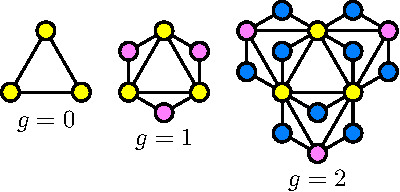
\includegraphics[width=0.75\linewidth]{Pseudofractal-eps-converted-to.pdf}
    \caption{ Illustration of the first several iterations of the pseudofractal scale-free web. }
    \label{psfw1}
\end{figure}
%%%%%%%%%%%%%%%%%%%%%%%%%%%%%%%%%%%%%%%%%%%%%%%%%%%%%%%%%%


The Koch network is also built in an iterative way. Let \(\mathcal{M}_{g}\) (\(g \geq 0\)) denote the Koch network after \(g\) iterations. Initially (\(g=0\)), \(\mathcal{M}_{0}\) is a triangle with three
vertices and three edges. For \(g\geq 1\), \(\mathcal{M}_{g}\) is obtained from \(\mathcal{M}_{g-1}\) by
performing the following operations. For each of the three vertices in
every existing triangle in \(\mathcal{M}_{g-1}\), two new vertices are created, both of which and their
``mother'' vertices are connected to one another forming a new triangle. Figure~\ref{network} illustrates the growth process of the Koch network.  In network \(\mathcal{M}_{g}\), the number of vertices is \(2\times 4^{g}+1\), and the number of
edges is \(3\times 4^{g}\).  In~\cite{XiLiZh15}, the Kemeny constant \(K(\mathcal{M}_g)\) for \(\mathcal{M}_g\) was obtained to be
\begin{equation}\label{Kg02}
    K(\mathcal{M}_g)=(1+2g)\times 4^g+\frac{1}{3}\,. %\notag
\end{equation}

%%%%%%%%%%%%%%%%%%%%%%%%%%%%%%%%%%%%%%%%%%%%%%%%%%%%%%%%%
% Figure 2
%%%%%%%%%%%%%%%%%%%%%%%%%%%%%%%%%%%%%%%%%%%%%%%%%%%%%
\begin{figure}[!t]
    \centering
    % \includegraphics[width=0.85\linewidth,trim=0 0 0 0]{Koch.eps}
    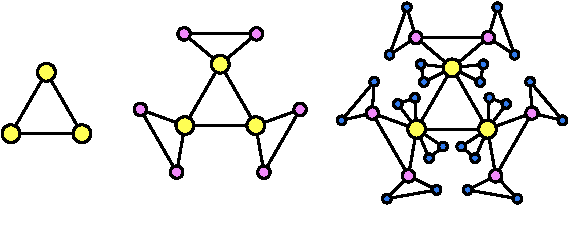
\includegraphics[width=0.85\linewidth]{Koch-eps-converted-to.pdf}
    \caption{Construction process for the Koch network.}
    \label{network}
\end{figure}
%%%%%%%%%%%%%%%%%%%%%%%%%%%%%%%%%%%%%%%%%%%%%%%%%%%%%

We use our  algorithm \(\text{Approx}\mathcal{HK}\) to compute the Kemeny constant on  pseudofractal scale-free web \(\mathcal{F}_{12}\) and the Koch network \(\mathcal{M}_{10}\). The numerical results are reported in  Table~\ref{tab:Kemeny}, which shows that the approximation algorithm \(\text{Approx}\mathcal{HK}\) works effectively for both networks. This again demonstrates the advantage of our proposed algorithm for large networks.

%%%%%%%%%%%%%%%%%%%%%%%%%%%%%%%%%%%%%%%%%%%%%%%
\begin{table*}[htbp]
    %\tabcolsep=5pt
    \centering
    \normalsize
    %\fontsize{6.51}{8.0}\selectfont
    \begin{threeparttable}
        \caption{Exact Kemeny constant \(K\),   their approximation \(\tilde{K}\),  relative error \(\rho=(K-\tilde{K})/K\), and running time (seconds, \(s\)) for \(\tilde{K}\) on networks \(\mathcal{F}_{12}\) and \(\mathcal{M}_{10}\).  \(K\) is obtained via~\eqref{Kg01} and~\eqref{Kg02}, while \(\tilde{K}\) is obtained through algorithm \(\text{Approx}\mathcal{HK}\) with \(\epsilon=0.1\).}
        \label{tab:Kemeny}
        \begin{tabular}{ccccccc}
            \toprule
            Network              & Vertices  & Edges     & \(K\)      & \(\tilde{K}\) & Error \(\rho\) & Time\cr
            \midrule
            \specialrule{0em}{3pt}{3pt}
            \(\mathcal{F}_{12}\) & 797,163   & 1,594,323 & 1,321,776  & 1,321,956     & 0.00014        & 207\cr
            \specialrule{0em}{3pt}{3pt}
            \(\mathcal{M}_{10}\) & 2,097,153 & 3,145,728 & 22,020,096 & 22,018,022    & 0.000094       & 1917\cr
            \specialrule{0em}{3pt}{3pt}
            %ZGL	           & 1,594,324  & 1,594,323  & 14,348,907 & 14,341,659\cr
            %\specialrule{0em}{3pt}{3pt}
            %ABZ			& 1,572,862  & 1,572,861 & 52,953,206 & 53,010,203\cr
            %\specialrule{0em}{3pt}{3pt}
            %DA			& 2,125,764  & 3,188,646 & 975,712,194 & 959,864,749\cr
            \bottomrule
        \end{tabular}
    \end{threeparttable}
\end{table*}
\section{Conclusions}

The hitting time of random walks arises  in many practical scenarios. However, the time cost of exactly computing hitting time is prohibitively expensive. In this paper, we studied a walk centrality and Kemeny constant of a graph, both of which are actually weighted average of hitting times and have found wide  applications. We established a link between the two quantities, and reformulated them in terms of quadratic forms of the pseudoinverse of graph Laplacian. Moreover, we provided a randomized approximation algorithm with probabilistic guarantee, which computes the walk centrality for all vertices and Kemeny constant in nearly linear time with respect to  the number of edges. Finally, we conducted extensive experiments on various real-world and model networks, which show that the proposed  algorithm is both efficient and accurate, especially for large-scale networks. %It is expected that our approximate method can be extended or modified to compute other quantities derived from hitting times~\cite{Lo93}.

\bibliographystyle{IEEEtran}
\balance
\bibliography{refs}

\end{document}
